\begin{document}
\chapter{Results}
\section{Error and convergence from simulated data} \label{simDataError}
The results of the simulations on the influence of noise on the global estimator, explained in section \ref{ch:simulationOfData} are presented in this section.
\subsection{Convergence of estimate for noise free measurements with different initial error}
The results of simulations of the convergence of the state estimates $\boldsymbol \theta$ as a function of the number of iterations for is shown in figure \ref{fig:sim_est_pos_conv}.
The simulations with initial estimate error were found to converge with an initial estimate error in the position of magnitude up to $10^7$m in all directions. The error in the final estimate is in the order of $10^{-7}$. 
%This is larger than the 16 digits of precision used by MATLAB by default. These results are assumed to be due to observations being in the range of approximately 2$\sim$3$\cdot 10^7$ m making an observation registered with eight digits of precision.
When adding noise to the satellite position or to the observations, a random noise is added to the satellite position of increasing magnitude from 1 to $10^4$ m. These simulations indicate that the estimator behaves as expected since the final error grows equal to the noise.
\par 
\begin{figure}[!h]
    \centering % <-- added
\begin{subfigure}{0.8\textwidth}
  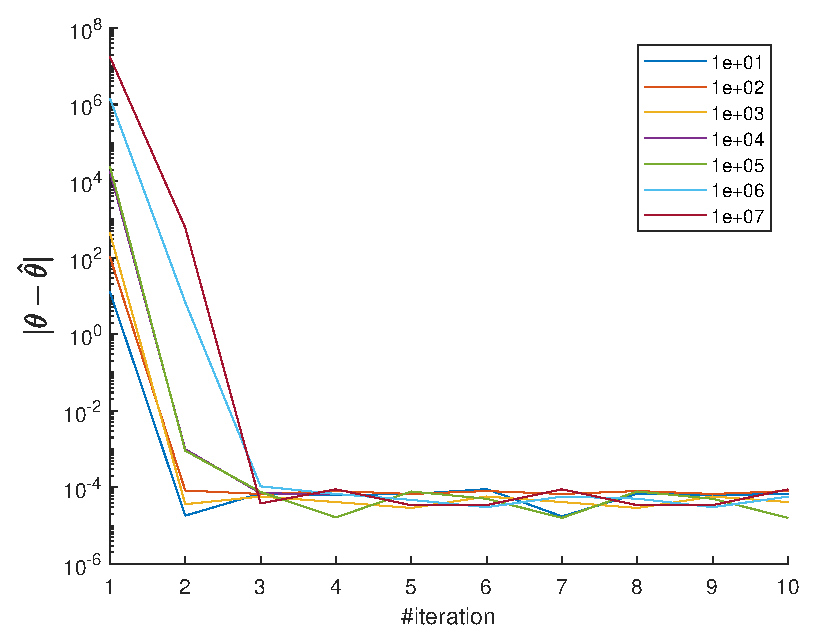
\includegraphics[width=\linewidth]{Results/SimulationEstPos/noiseFreeConv}
  \subcaption{Convergence of estimate error with a growing error in the initial position estimate.}
\end{subfigure}
\begin{subfigure}{0.8\textwidth}
  \includegraphics[width=\linewidth]{Results/SimulationEstPos/clockBConv}
    \subcaption{Convergence of estimate error with a growing receiver clock bias. Plot is split to show error in position (upper) and in clock bias (lower).}
\end{subfigure}
\end{figure}
\begin{figure}\ContinuedFloat
\begin{subfigure}{0.8\textwidth}
  \includegraphics[width=\linewidth]{Results/SimulationEstPos/satPosConv}  
    \subcaption{Convergence of estimate error with a growing error in calculated satellite position.}
\end{subfigure}
\begin{subfigure}{0.8\textwidth}
  \includegraphics[width=\linewidth]{Results/SimulationEstPos/GaussianConv}
    \subcaption{Convergence of estimate error with a growing added observation noise.}
\end{subfigure}
\caption{Simulation results with different input noise. The horizontal axis shows the number of iterations and vertical axis shows the norm of the error, where the estimate is indicated with a $\wedge$-symbol and the true value in the simulation without. Magnitude of the noise is indicated in the legend.} 
\label{fig:sim_est_pos_conv}
\end{figure}
\begin{comment}
\begin{figure}[!h]
    \centering % <-- added
\begin{subfigure}{0.8\textwidth}
  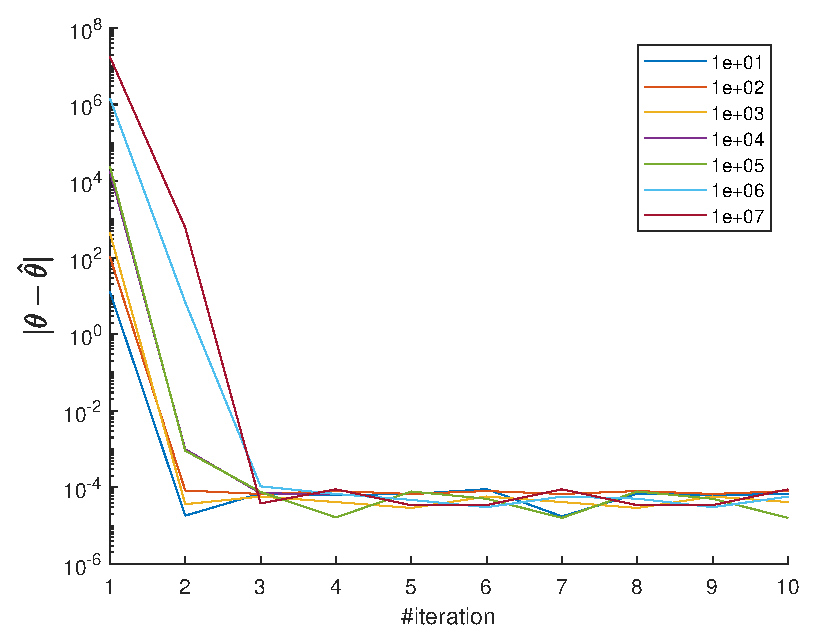
\includegraphics[width=\linewidth]{Results/SimulationEstPos/noiseFreeConv}
  \subcaption{A}
\end{subfigure}
\begin{subfigure}{0.8\textwidth}
  \includegraphics[width=\linewidth]{Results/SimulationEstPos/clockBConv}
  \subcaption{B}
\end{subfigure}
\end{figure}
\begin{figure}\ContinuedFloat
\begin{subfigure}{0.49\textwidth}
  \includegraphics[width=\linewidth]{Results/SimulationEstPos/satPosConv}  
    \subcaption{C}
\end{subfigure}
\begin{subfigure}{0.49\textwidth}
  \includegraphics[width=\linewidth]{Results/SimulationEstPos/GaussianConv}
    \subcaption{D}
\end{subfigure}
\caption{Simulation results with different input noise. From top left to bottom right: a)Noise free, b) Clock bias, c) Satellite position, f) Gaussian noise. In figure a), different error in starting positions is tested. The horizontal axis shows the number of iterations and vertical axis shows the norm of the error between true and estimated states $|{\boldsymbol \theta}-\hat{{\boldsymbol \theta}}|$.} 
\label{fig:sim_est_pos_conv}
\end{figure}
\end{comment}
In figure \ref{fig:mixedConv} the convergence of an erroneous initial state with an added clock bias is presented. For any magnitude of initial error in all parameters between $10^{-10}$ to $10^4$ m the parameters converge to the correct value within the interruption threshold of the estimator function.

\begin{figure}[htb]
    \centering % <-- added
  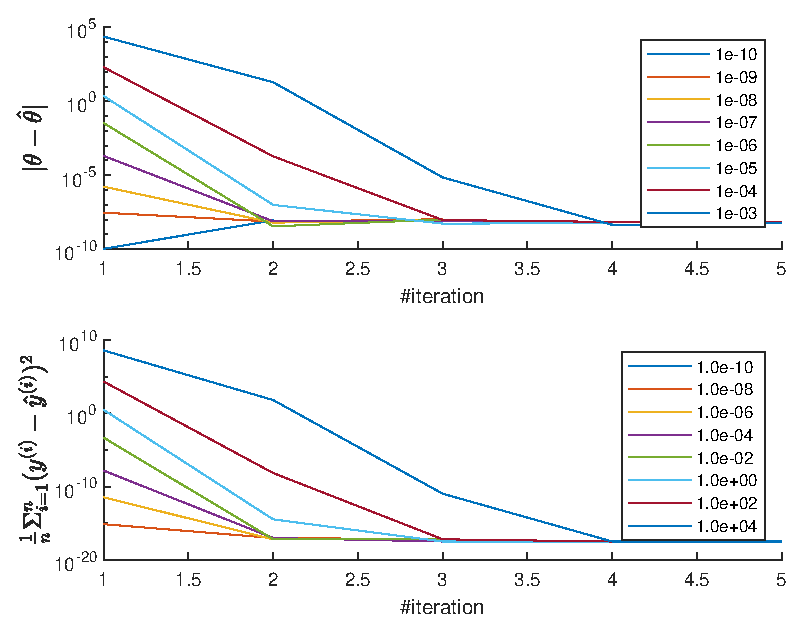
\includegraphics[width=0.8\linewidth]{Results/SimulationEstPos/mixedNoiseConv}
\caption{\label{fig:mixedConv} The plots show the convergence behaviour with noise free estimates and an initial random error in both position and clock bias of increasing magnitude. Upper: norm of error in state estimate per iteration. Lower: mean square error in estimated observations. $\wedge$-symbol indicates an estimate.}
\end{figure}	

\subsection{Final estimate for added measurement noise of different magnitudes}
The simulated error in the terminal estimate of receiver states when adding noise of increasing magnitude is presented in figure \ref{fig:sim_est_pos}. In the upper graph, three types of error in the estimates are shown: the norm of error in position, the norm of error in position and clock bias and the mean square error in the observations.
%$|\bf p-\hat{p}|$, ${|{\boldsymbol \theta}-\hat{{\boldsymbol \theta}}|}$ and $\frac{1}{n}\sum (y-\hat{y}))^2$ where a simulated observation is produced as that given in equation (\ref{ObsRange}), and thus $\hat{y}$ is the predicted measurement given the calculated satellite's position and estimated state of the receiver from equation (\ref{hModel}). \\
\begin{figure}[!h]
    \centering % <-- added
\begin{subfigure}{0.8\textwidth}
  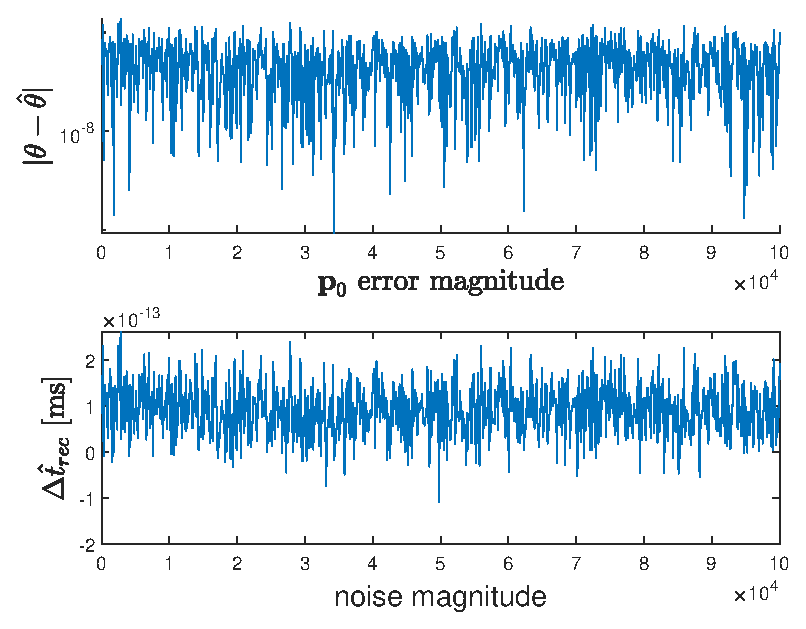
\includegraphics[width=\linewidth]{Results/SimulationEstPos/noiseFree}
  \subcaption{Error in final estimate for an initial position error. Error in state estimate (upper) and estimated receiver clock bias (lower)}
\end{subfigure}
\begin{subfigure}{0.8\textwidth}
  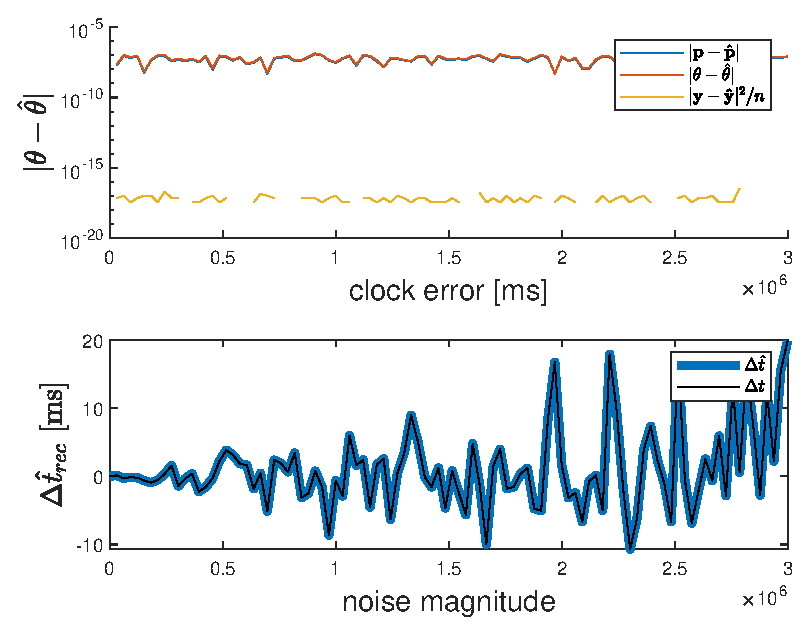
\includegraphics[width=\linewidth]{Results/SimulationEstPos/clockB}
  \subcaption{Error in final estimate for a receiver clock bias. Error in state estimate (upper) and true and estimated receiver clock bias (lower).}
\end{subfigure}
\end{figure}
\begin{figure}\ContinuedFloat
\begin{subfigure}{0.8\textwidth}
  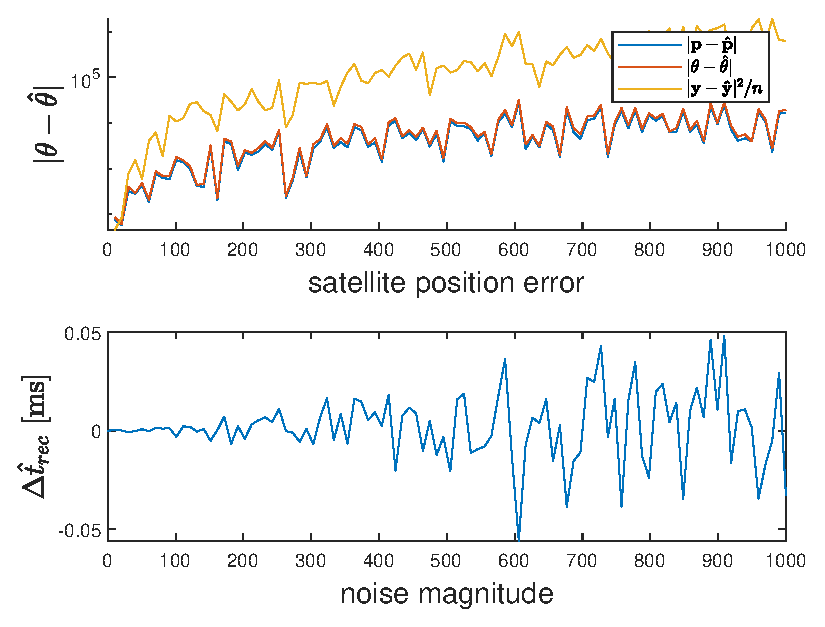
\includegraphics[width=\linewidth]{Results/SimulationEstPos/satPos}  
	\subcaption{Error in final estimate with added satellite position error. Error in state estimate (upper) and estimated receiver clock bias (lower).}
\end{subfigure}
\begin{subfigure}{0.8\textwidth}
  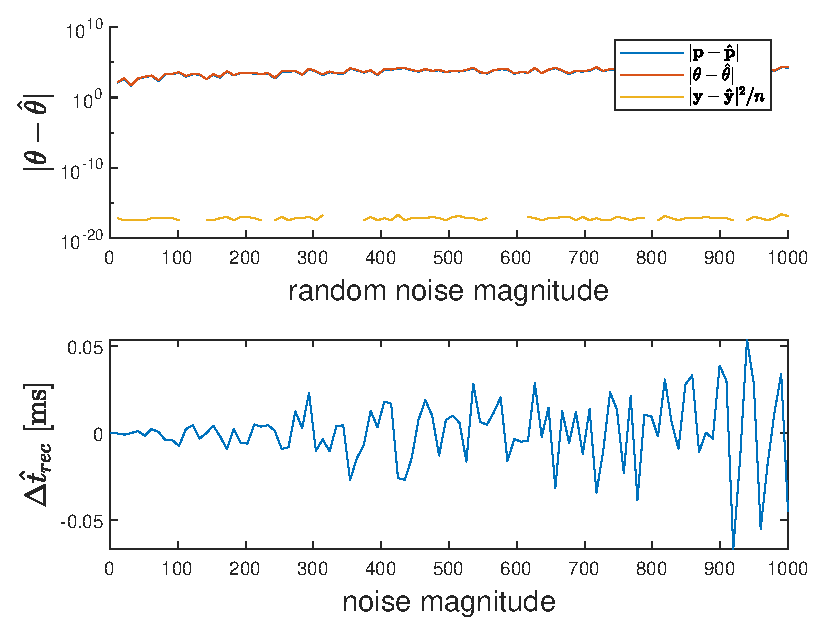
\includegraphics[width=\linewidth]{Results/SimulationEstPos/Gaussian}
  \subcaption{Error in final estimate with added observation noise. Error in state estimate (upper) and estimated receiver clock bias (lower).}
\end{subfigure}
\caption{Simulation results with input noise of growing magnitude. Estimates are denoted with a $\wedge$-symbol, and true values without. The upper figure in each pair shows the norm of the error in position estimate, error in receiver state estimate and mean error in range estimate with a growing magnitude of the noise. In b), the true and estimated receiver clock bias are plotted together. Gaps in range error graph is due to round off error as value is close to zero.}
\label{fig:sim_est_pos}
\end{figure}
\par
The simulations show that for an error consisting only of receiver clock bias, the effect on the positioning is negligible, as $|\textbf{p}-\hat{\textbf{p}}|$ lies steadily around $10^{-10}$. For other types of added noise, the error appear to grow at the same rate as that of the noise source. This is an indication that the estimator functions as intended for simulated data.

\subsection{Comparison of RMSE of relative position from simulated data}\label{RMSEsim}
Simulations of the global position estimator and DD-estimator are done as described in section \ref{RMSE} using a Gaussian white noise level of 1 m. The positions are calculated first using two independent global fixes, and then the DD relative position with an increasing magnitude the common noise. In figures (\ref{fig:Nsim1}-\ref{fig:Nsim20}) the simulated results are shown of increasing the magnitude of the common noise which is set to respectively 1, 10 and 20 m. 
\par
It's apparent that for the global positioning the error grows with the common noise, while the DD-estimate position appears to be unaffected. This motivates the use of the DD-method for high levels of the common noise $\eta$ shared between the receivers.
\begin{figure}[!htb]
%\begin{centering}
\begin{subfigure}{\textwidth}
\includegraphics[width=\textwidth]{Results/MSEplots/Esim1.eps}
\subcaption{\label{fig:Nsim1} Common noise scaled by a factor 1.}
%\caption{\label{fig:Nsim2} Result of relative position from global position fixes (upper) and DD relative position (lower) using simulated data with a magnitude of 1 for the bias.}
\end{subfigure}
\begin{subfigure}{\textwidth}
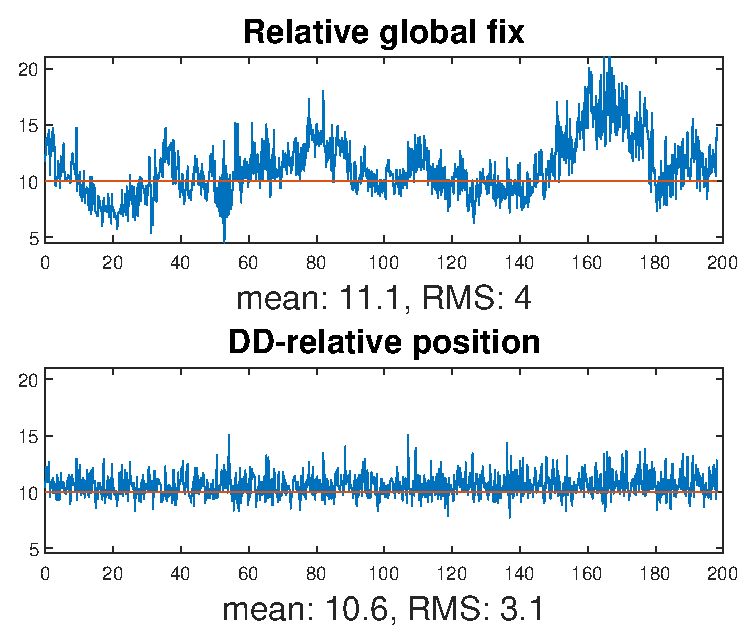
\includegraphics[width=\textwidth]{Results/MSEplots/Esim10.eps}
\subcaption{\label{fig:Nsim10} Common noise scaled by a factor 10.}
%\caption{\label{fig:Nsim10} Result of relative position from global position fixes (upper) and DD relative position (lower) using simulated data with a magnitude of 10 for the bias.}
\end{subfigure}
\end{figure}
\begin{figure}[!htb]\ContinuedFloat
\begin{subfigure}{\textwidth}
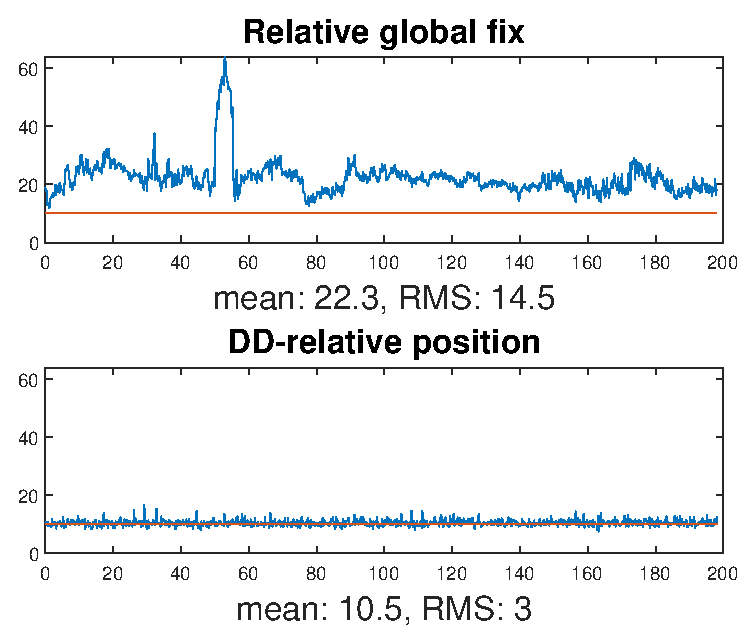
\includegraphics[width=\textwidth]{Results/MSEplots/Esim20.eps}
\subcaption{\label{fig:Nsim20} Common noise scaled by a factor 20.}
%\caption{\label{fig:Nsim20} Result of relative position from global position fixes (upper) and DD relative position (lower) using simulated data with a magnitude of 20 for the bias.}
\end{subfigure}
\caption{RMSE of global position and DD estimator from simulated data. The common noise $\eta^{(i)}$ for a satellite $i$ is randomly sampled and scaled as indicated in the respective figure.}
%\end{centering}
\end{figure}


\begin{comment}
\section{Calculating satellite position}\label{satelliteTrajectory}
The satellite positions are calculated in accordance with the method described in section \ref{chap:ephPositioning}. The position is presented in two forms, the position in the sky over time in a polar chart without any corresponding time stamp, as well as 1D graphs of  elevation with regards to the position of the receiver given by the onboard electronics. For measurements taken on April 11, 2019, starting at 12:25:28 (UTC), the skyplot of the calculated satellite positions are shown in figure \ref{fig:skyplot}, next to that available at online source\footnote{link to reconstruct plot: 
\url{https://www.gnssplanning.com/\#/embedded?satellites=1,2,3,5,6,7,8,9,10,11,12,13,14,15,16,17,18,19,20,21,22,23,24,25,26,27,28,29,30,31,32&satSystems=GPS&restoreSats=0&target=settings&cutoffDeg=0&durationHours=6&utcTime=2019-04-11T12:00:00&hgt=10&lonDeg=18.0687918056&latDeg=59.3481576111}
}
\begin{figure}
\begin{minipage}{0.49\textwidth}
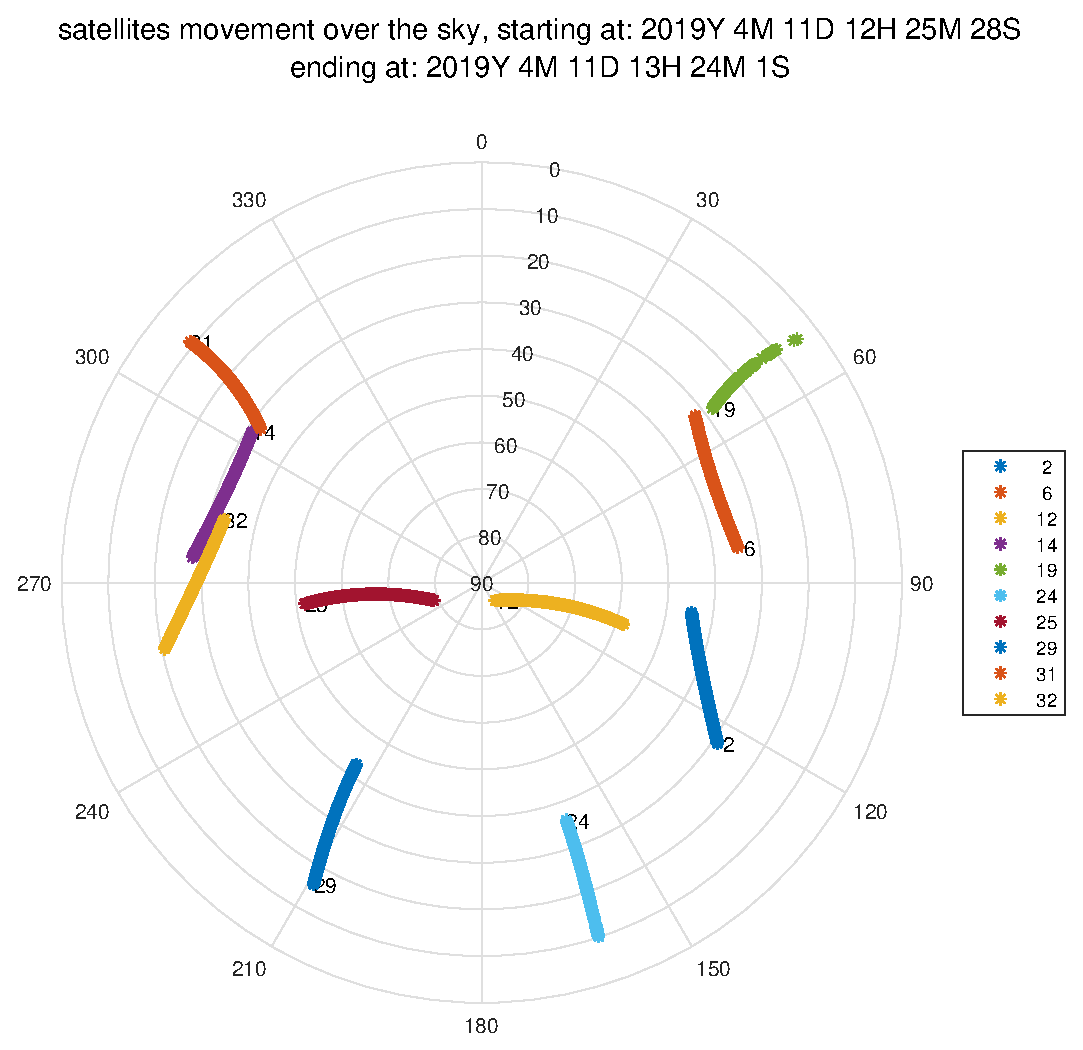
\includegraphics[width=\textwidth]{Results/satsInSky.eps}
\caption{\label{fig:skyplot} GPS Satellite's movement in the sky for the duration of the measurement, only showing when they are observed by the receiver.}
\end{minipage}
\begin{minipage}{0.49\textwidth}
\vspace{3 mm}
\includegraphics[width=\textwidth]{Results/skyplot190411-1230}
\caption{\label{fig:skyplotGNSSPLANNING} Skyplot for all visible GPS-satellites at UTC 2019-04-11, 12:30 Stockholm, Sweden from \url{www.gnssplanning.com}. Trajectories indicated without direction}
\end{minipage}
\end{figure}
The elevation, azimuth and distance calculations for the GPS satellites over the same time interval as indicated in figure \ref{fig:skyplot} is shown in figure \ref{fig:el6H}. The corresponding elevation over time for the satellites in figure (\ref{fig:skyplotGNSSPLANNING}) is shown in figure \ref{fig:elGNSSPlanning}. Note that the time interval is larger in figure \ref{fig:elGNSSPlanning} than that of \ref{fig:el6H} due to only actually sampled satellite ephemeris data is used and satellites only being visible for a short time period. 
\par 
A coarse evaluation indicates that the solutions are equal. The precision with which the satellite positions can be evaluated is however quite low with regards to a fine positioning solution.
\begin{figure}[!h]
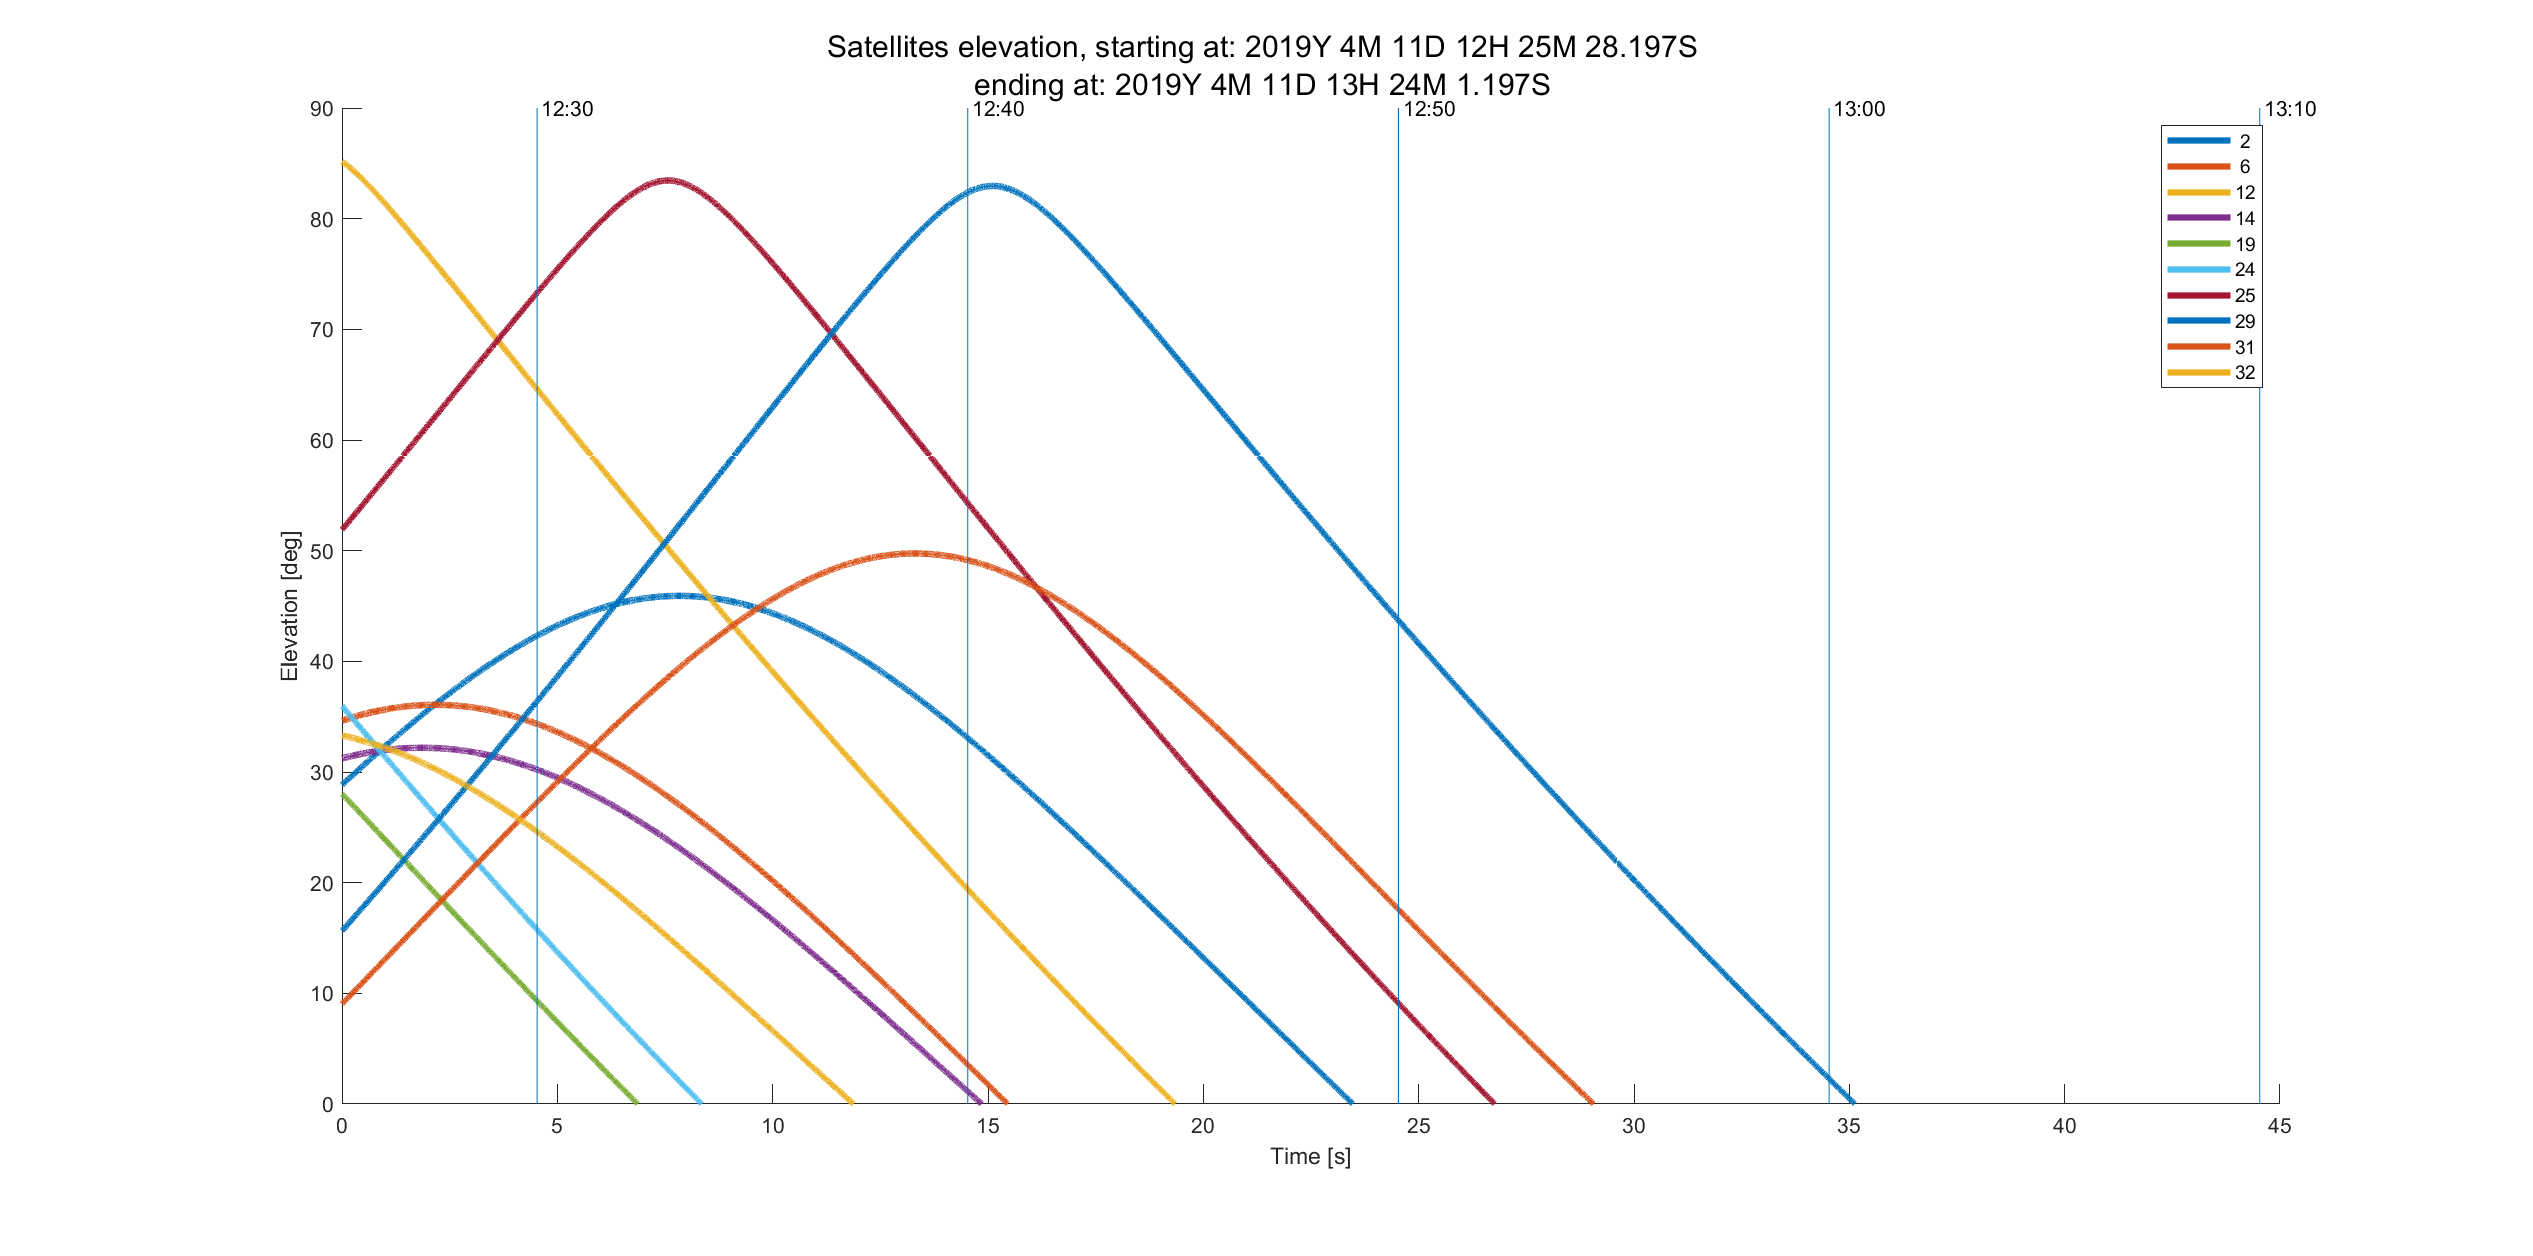
\includegraphics[width=\textwidth]{Results/elev6H.eps}
\caption{\label{fig:el6H} Elevation (upper), Azimuth (middle) Distance (lower) for GPS-satellites with regards to receiver at position 59.353$^o$N, 18.073$^o$E.}
\end{figure}
\begin{figure}
\centering
\includegraphics[width=0.7\textwidth]{Results/elevGNSSPlanning.jpg}
\caption{\label{fig:elGNSSPlanning} Elevation plot from \url{gnssplanning.com} at coordinates 59.353$^o$N, 18.073$^o$E. }
\end{figure}
\end{comment}

\section{Individual and relative position estimate using global positioning}
This section presents the results of the onboard estimate and the global position estimator, where positions are calculated individually. Sampling was performed for approximately 30 minutes per receiver in each direction. The results are presented in the form of:
\begin{itemize}
\item A histogram of the position estimate per direction per receiver.
\item A plot of the position over time per direction.
\item A table showing relative position and standard deviation.
\end{itemize}
\subsection{Position from onboard estimate} \label{onBoardSolution}
The two individual onboard estimates is illustrated as a histogram in figures \ref{fig:histN}-\ref{fig:histE} from a approximately 8500 samples per receiver.
\begin{figure}
\centering
\begin{subfigure}{\textwidth}
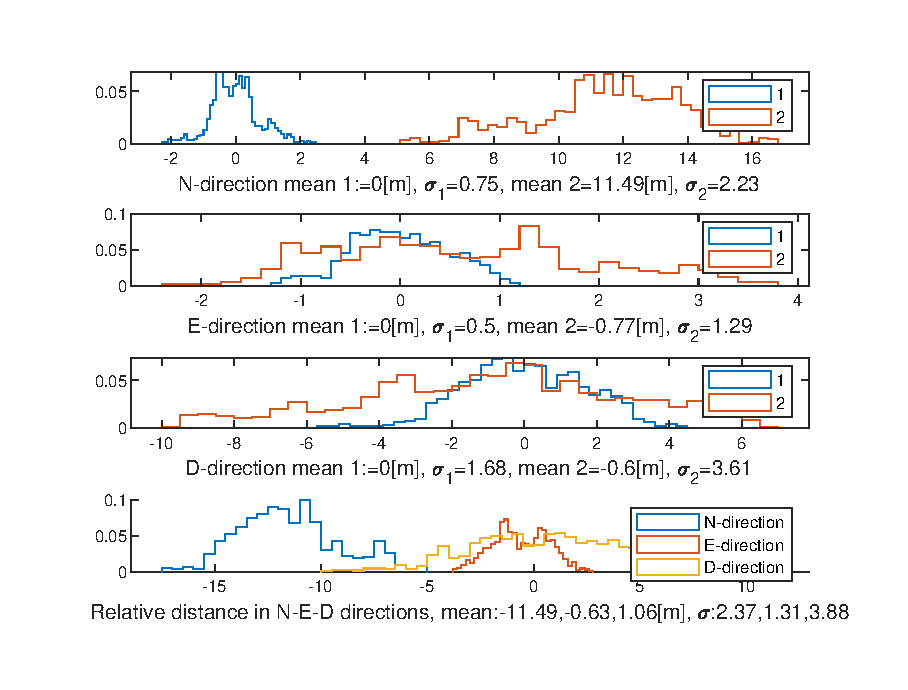
\includegraphics[width=\textwidth]{Results/GPShist10mN.eps}
\subcaption{\label{fig:histN} Histogram over position estimate with an east direction separation.}
%Histogram over position over time with an East direction baseline of 10 m separate per direction, N-direction (upper), E-direction (second from top), D-direction (second from bottom), Relative distance for all three directions at synchronised times (bottom).}
\end{subfigure}
\begin{subfigure}{\textwidth}
\centering
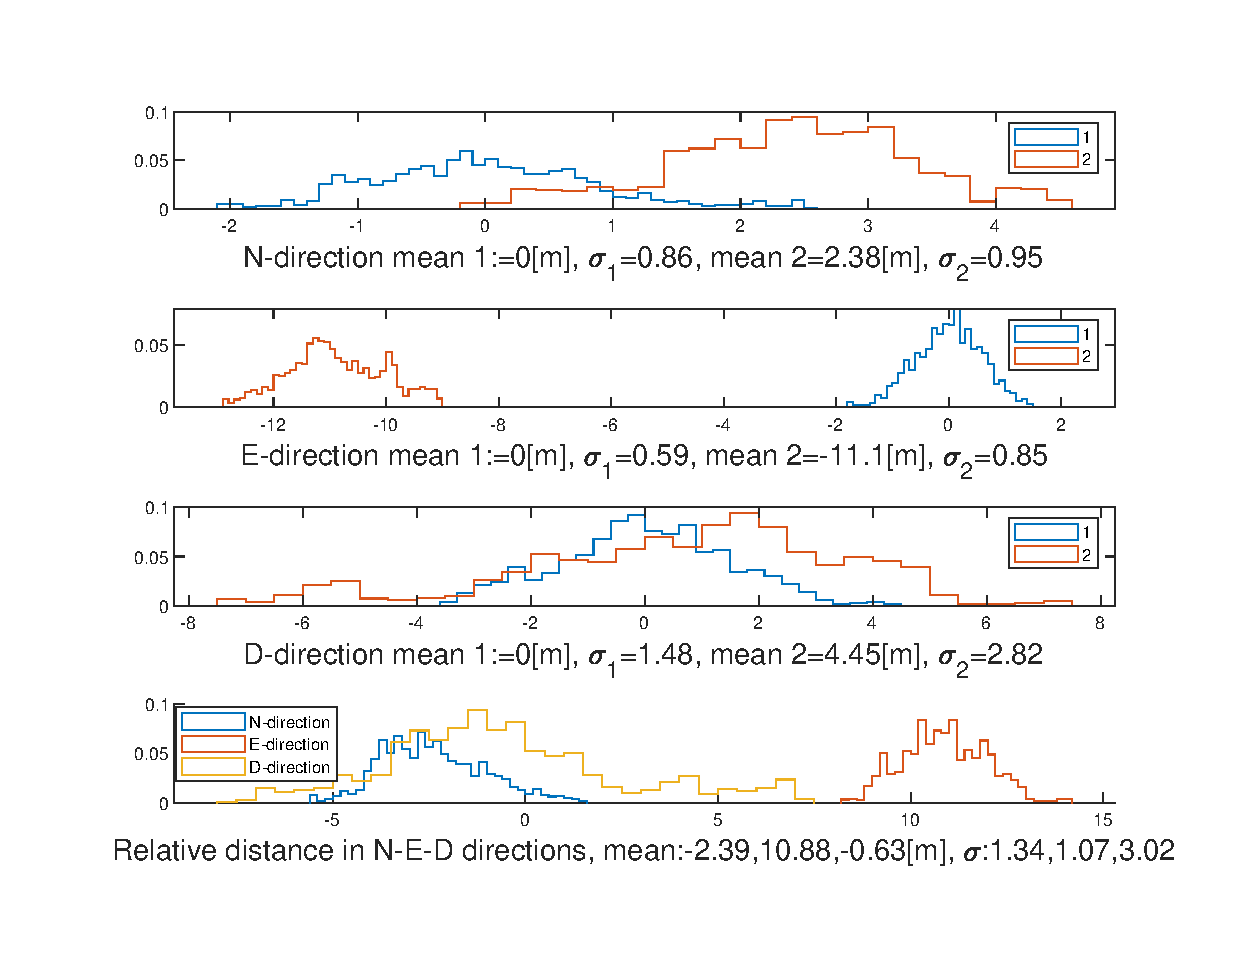
\includegraphics[width=\textwidth]{Results/GPShist10mE.eps}
\subcaption{\label{fig:histE} Histogram over position estimate with a north direction separation.}
%Histogram over position over time with an North direction baseline of 10 m separate per direction, N-direction (upper), E-direction (second from top), D-direction (second from bottom), Relative distance for all three directions at synchronised times (bottom)}
\end{subfigure}
\caption{Histogram showing position estimate over time with a baseline of 10 m separation between receivers from onboard estimate. For both figures: N-direction (upper), E-direction (second from top), D-direction (second from bottom), relative distance for all three directions at synchronised times (bottom). Origin is set to the first estimate of receiver 1.}
\end{figure}
The estimate is transformed from an ECEF frame to a NED frame using the first registered position from receiver 1. Here the origin has been set to the mean over time for receiver 1 per direction. The ideal outcome would be positions separated by 10 m in one direction and 0 in the others and have a Gaussian distribution. 
\par
The standard deviation per direction and observation series is presented in table \ref{table:resultsHistIS}. $\sigma_{12}$ has been introduced to denote the standard deviation in the relative estimate between the receivers. It is apparent from the images and the data in the table that the standard deviation of receiver 2 is greater than that of receiver 1 for all directions in both observations. It can be noted that receiver 2 is that which was placed close to the pin in figure \ref{fig:Uggleviken} and was closer to the forest right north of it than receiver 1 for both observations.
\begin{table}[h!]
  \begin{center}
    \begin{tabular}{|c|c|c|c|}\hline
		& \textbf{North} & \textbf{East}& \textbf{Down}\\
      \hline
      	E-dir \\ \hline
      	$\Delta p $ [m]& -11.5 & -0.6 & 1\\ \hline
		$\sigma_1$& 0.8 & 0.5 & 1.7 \\\hline
		$\sigma_2$ & 2.2 & 1.3 & 3.6 \\ \hline
		$\sigma_{12}$& 2.4 & 1.3 & 3.9 \\ \hline
		N-dir\\ \hline
		$\Delta p $ [m]& -2.4& 10.9 & -0.6 \\ \hline
		$\sigma_1$& 0.9 & 0.6 & 1.5 \\\hline
		$\sigma_2$ & 1 & 0.9 & 2.8 \\ \hline
		$\sigma_{12}$ & 1.3 & 1 & 3 \\ \hline
    \end{tabular}
    \caption{\label{table:resultsHistIS} Mean and standard deviation of position from on board individual estimate, as well as the relative estimate. Values referring to the figures \ref{fig:histN}-\ref{fig:histE}}
  \end{center}
\end{table}

\subsection{Global and relative position estimates from global position estimator}\label{leastSquareEstimator}
The global position for two receivers is calculated as described in section \ref{stateEst} from received ephemeris and observation data. The observations are weighted using their respective SNR-value as described in equation (\ref{SNRWeights}).
The results are based on approximately 8500 samples per receiver and observation series. They are presented in two ways:
\begin{itemize}
\begin{samepage}
\item The positions are calculated independently for the receivers, using all available satellites.
\item Only satellites which are shared between receivers are used.
\end{samepage}
\end{itemize}
When fully independent estimates are used, several satellites may go in and out of tracking between two epochs, leading to a change in position estimate. The calculations when only shared information between receivers are used, only observations from satellites that were being tracked for the entirety of the observation series for both receivers were used and the rest discarded. The result of fully independent global estimates are presented in figures \ref{fig:globalPosAllSV}. The corresponding mean and standard deviation per direction for the two observations are presented in table \ref{table:resultsPosAllSat}. 
\par
The results of independent global estimates where only shared information is used is presented in \ref{fig:globalPosSelectSV} and the corresponding mean and standard deviation per direction are presented in table \ref{table:resultsPosSharedSat}. 
\par
The results from table \ref{table:resultsPosAllSat} and \ref{table:resultsPosSharedSat} are very similar, with a slightly higher error in position and standard deviation for the calculations where only shared information is used. As restricting the satellites to only using the shared information did not lead to improvements, no further results will be presented for this method.
\par
A comparison between the onboard estimate and that of the global position estimator indicates that the onboard estimate is still superior. The estimate over time per direction for the two sample series, where they have been plotted together are shown in figure \ref{fig:onboardAndGlobal}. The position estimates from the onboard estimate and the global estimates from observation data are mostly very close and following the same trend, meaning that the estimates change similarly over time. It is however apparent that for some observations, the difference between the estimates becomes very large, in the order of several meters, as well as that the noise levels of the global position estimator are much larger than that of the onboard estimate. 
\par
The difference between the solutions are assumed stemming primarily from two sources: that the onboard estimate is filtered, as well as that it estimates the atmospheric noise. The filtering is indicated by that the position estimate follows a smooth curve without jumps between epochs. It is also likely that the ionospheric noise is estimated in the onboard position estimates. This has the potential to reduce the both the global and relative error significantly under the assumption that the noise is a common noise to both receivers, as shown in simulations in section \ref{RMSEsection}.
\begin{figure}[H]
\begin{subfigure}{\textwidth}
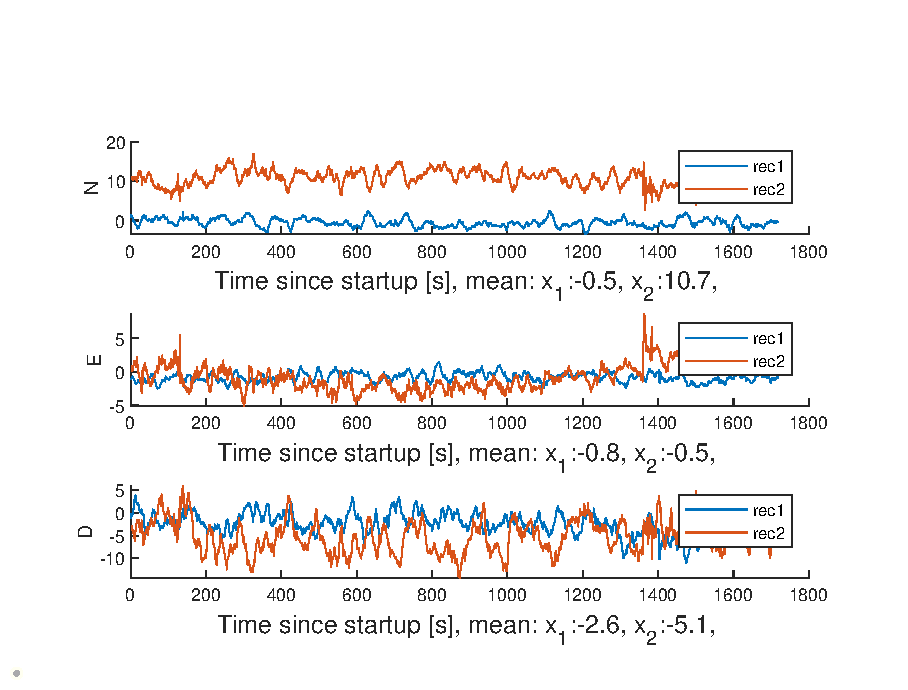
\includegraphics[width=1\textwidth]{Results/DistNED30MinNAllSat}
\subcaption{Position estimate in a NED-frame for separated by a 10 m baseline in a north direction.}
\end{subfigure}
\begin{subfigure}{\textwidth}
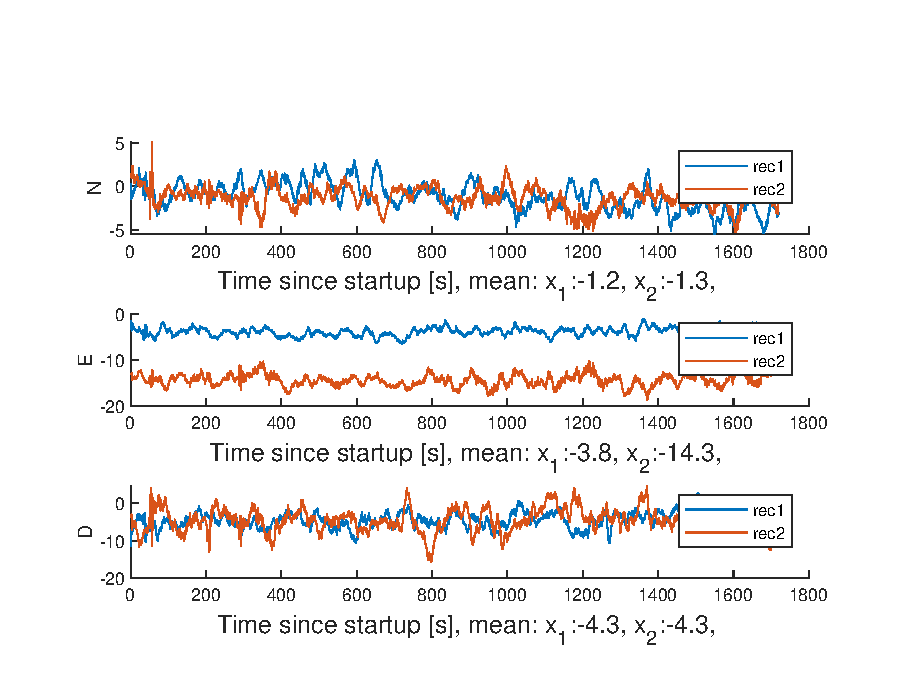
\includegraphics[width=1\textwidth]{Results/DistNED30MinEAllSat}
\subcaption{Position estimate in a NED-frame for separated by a 10 m baseline in an east direction.}
\end{subfigure}
\caption{\label{fig:globalPosAllSV} Independent global position estimates for two receivers separated 10 m in N, E and D directions respectively. The origin is set to the first onboard estimate of receiver one. All satellite information known to respective receiver is used.}
\end{figure}
\begin{table}[h!]
\begin{minipage}{0.45\linewidth}
  \begin{center} 
    \begin{tabular}{|c|c|c|c|}\hline
		& \textbf{North} & \textbf{East}& \textbf{Down}\\
      \hline
      	E-dir \\ \hline
      	$\Delta p $ [m]& 10.2 & 0.3 & -2.6\\ \hline
		$\sigma_1$& 1.6 & 0.9 & 2.2 \\\hline
		$\sigma_2$ & 1.2 &1.3 & 3.3 \\ \hline
		$\sigma_{12}$ & 2.3 & 1.8 & 4.2 \\ \hline
		N-dir\\ \hline
		$\Delta p $ [m]& -0.1& -10.5 & 0 \\ \hline
		$\sigma_1$& 1 & 0.7 & 2.4 \\\hline
		$\sigma_2$ & 2 &2.1 & 3.5 \\ \hline
		$\sigma_{12}$ & 2.5 & 3.3 & 5.5 \\ \hline
	\end{tabular}
    \subcaption{\label{table:resultsPosAllSat} Values calculated for when receivers use all available information. Values referring to observation series shown in figure \ref{fig:globalPosAllSV}.}
  \end{center}
\end{minipage}
\hfill
\begin{minipage}{0.45\linewidth}
  \begin{center}
    \begin{tabular}{|c|c|c|c|}\hline
		& \textbf{North} & \textbf{East}& \textbf{Down}\\
      \hline
      	E-dir\\ \hline
      	$\Delta p $ [m]& 10.6& 0.6 & -1 \\ \hline 
		$\sigma_1$& 1.8 & 1.4 & 2.5 \\\hline
		$\sigma_2$ & 1.4 &1.3 & 3.8 \\ \hline
		$\sigma_{12}$ & 2.2 & 1.9 & 4.3 \\ \hline
		N-dir\\ \hline
		$\Delta p $ [m]& -1.4 & -11.9 & -0.4 \\ \hline
		$\sigma_1$& 1 & 0.7 & 2.5 \\ \hline
		$\sigma_2$ & 2 &2.1 & 3.5 \\ \hline
		$\sigma_{12}$ & 3.7 & 3.5 & 5.5 \\ \hline
    \end{tabular}
    \subcaption{\label{table:resultsPosSharedSat} Values calculated for when only satellites shared between receivers are used. Values referring to observation series shown in figure \ref{fig:globalPosSelectSV}.}
  \end{center}
\end{minipage}
\caption{Averaged values of difference in position, standard deviation of  position estimate per direction and standard deviation of relative estimate.}
\end{table}

\begin{figure}[H]
\begin{subfigure}{\textwidth}
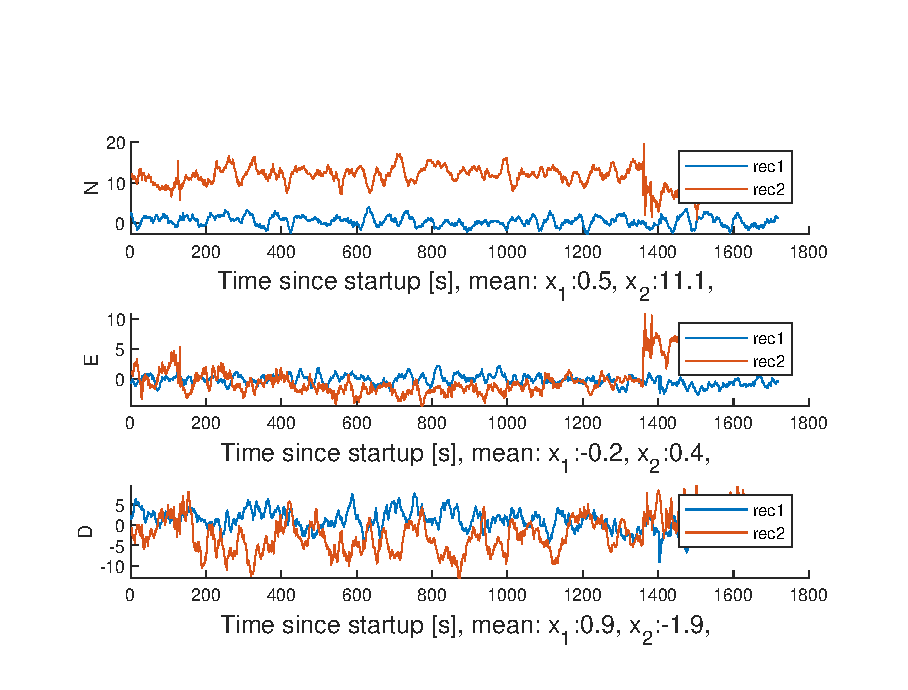
\includegraphics[width=1\textwidth]{Results/DistNED30MinNSharedSat}
\subcaption{Position estimate in a NED-frame for separated by a 10 m baseline in a north direction.}
\end{subfigure}
\begin{subfigure}{\textwidth}
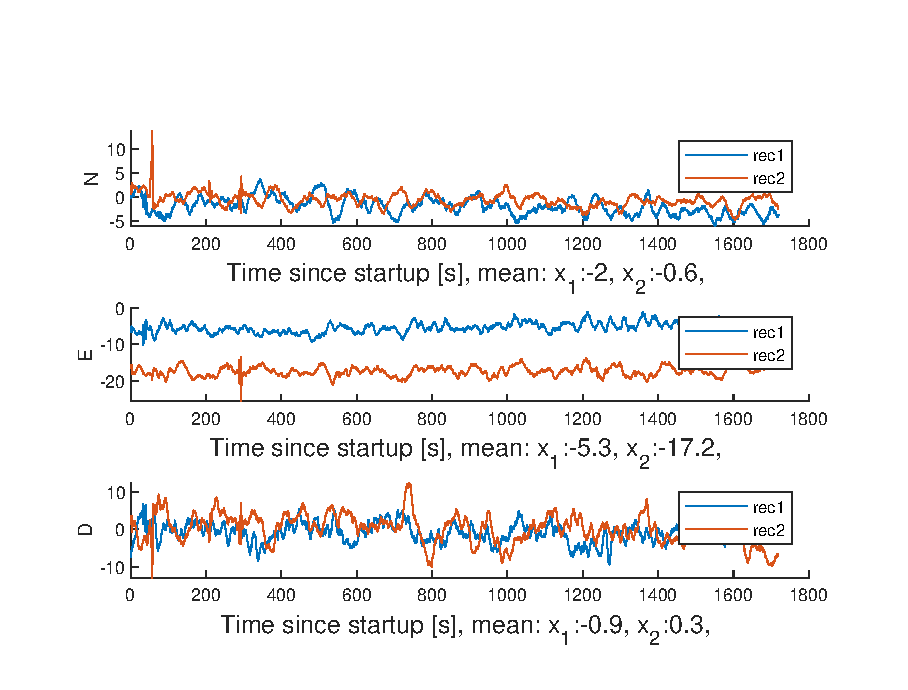
\includegraphics[width=1\textwidth]{Results/DistNED30MinESharedSats}
\subcaption{Position estimate in a NED-frame for separated by a 10 m baseline in an east direction.}
\end{subfigure}
\caption{\label{fig:globalPosSelectSV} Independent global position estimates for two receivers separated 10m N-direction (upper) and E-direction (lower), origin is set to true position. Only satellite data shared between receivers is used.}
\end{figure}

\section{Histograms of DD-relative position estimates}\label{histogramDD}
The DD-relative position estimates are calculated using the estimator described in section \ref{ch:DD_estimator}, using the observation weights in equation (\ref{DD_BLUE}). Histograms of the relative estimates per direction are shown in figures (\ref{fig:histRel1hN}-\ref{fig:histRel1hE}. The mean and standard deviation for each direction of the two sample periods is presented in table \ref{table:resultsRel}. The estimates use the same data as those used in section \ref{leastSquareEstimator}. 
\par
The relative estimates from the global position and DD-estimator are similar and the DD-estimator shows a slightly higher standard deviation for the north-direction observation and slightly lower for the east-direction. Using these results there is no directly discernible difference in the performance of the methods.
\par
The results from section \ref{onBoardSolution} is also compared those presented in figures (\ref{fig:histRel1hN}-\ref{fig:histRel1hE}) in figures (\ref{fig:DDandInternalN}-\ref{fig:DDandInternalE}). The plots clearly show that the standard deviation of the DD-estimate at best is equal to, or close to equal to that of the onboard solution but generally can be expected to be greater.

\begin{figure}[H]
\begin{subfigure}{\textwidth}
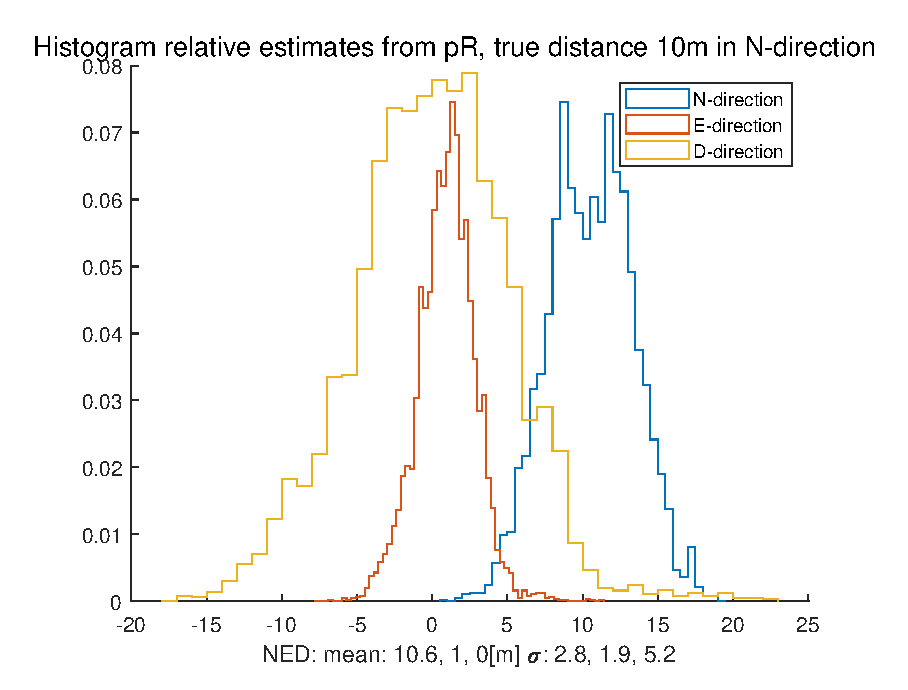
\includegraphics[width=\textwidth]{Results/histRel30MinN}
\subcaption{\label{fig:histRel1hN}}
%\caption{\label{fig:histRel1hN} Position over time with a North direction baseline of 10 m}
\end{subfigure}
\begin{subfigure}{\textwidth}
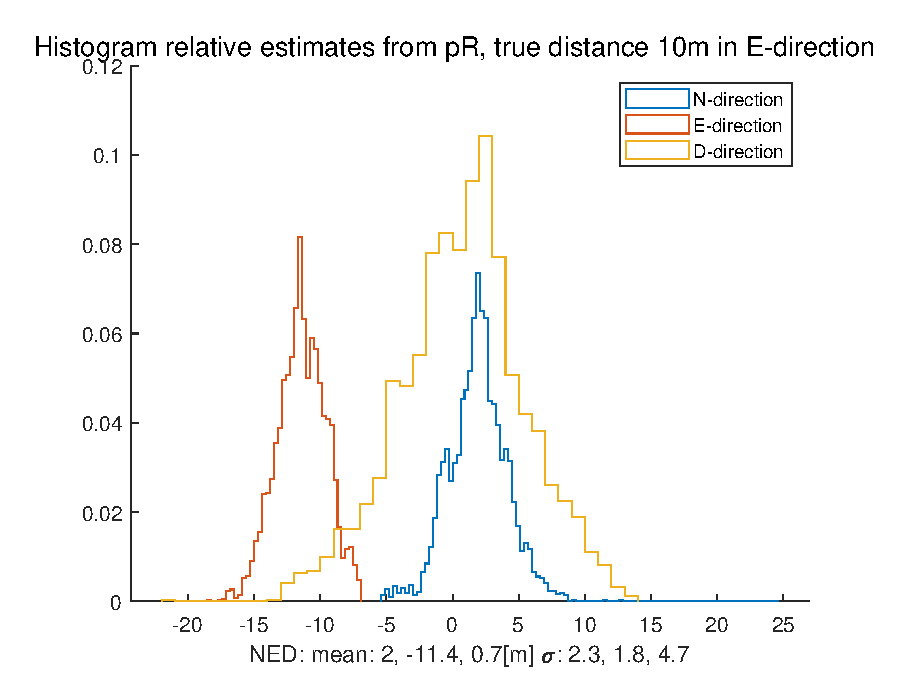
\includegraphics[width=\textwidth]{Results/histRel30MinE}
\subcaption{\label{fig:histRel1hE}}
%\caption{\label{fig:histRel1hE} Position over time with an East direction baseline of 10 m}
\end{subfigure}
\caption{Histogram over relative position estimate per direction from DD-estimator.}
\end{figure}

\begin{table}[!htb]
  \begin{center}
    \begin{tabular}{|c|c|c|c|}\hline
		& \textbf{North} & \textbf{East}& \textbf{Down}\\
      \hline
      True[m]& 10 & 0&0\\ \hline
      Mean[m] &10.6 & 1.0 & 0.0\\ \hline
		$\sigma$& 2.8 & 1.9 & 5.2 \\\hline
		True[m] & 0 &10&0\\ \hline
		Mean[m] & 1.1 & -10.1 & 1.0\\ \hline
		$\sigma$ & 2.0 &1.6 & 4.7 \\
		\hline
    \end{tabular}
    \caption{\label{table:resultsRel} Averaged values of difference in position and standard deviation of position estimate per direction for a DD-estimate. Values referring to measurements in figure (\ref{fig:histRel1hN}-\ref{fig:histRel1hE})}
  \end{center}
\end{table}

\section{RMSE of relative position from observation data}\label{RMSEsection}
The RMSE values of the relative estimates from observations, calculated in sections \ref{leastSquareEstimator} and \ref{histogramDD} are calculated. are shown in figures (\ref{fig:Nobs}-\ref{fig:Eobs}) with a 10 m separation in north and east direction separation respectively. 
\par 
The calculaed RMSE values are, respectively for the global position and DD estimator 5.6 and 4.9 m in north direction, and 5 and 4.8 in east direction. The DD-estimator thus performs slightly better in both cases. This result is expected from the simulations in section \ref{RMSEsim}, the decrease in error is however small. This indicates a higher level of random noise than expected in the observations.
\begin{figure}[!htb]
\centering
\begin{subfigure}{\textwidth}
\includegraphics[width=\textwidth]{Results/MSEplots/Nobs.eps}
\subcaption{\label{fig:Nobs} Receivers separated 10 m in north direction.}
\end{subfigure}
\begin{subfigure}{\textwidth}
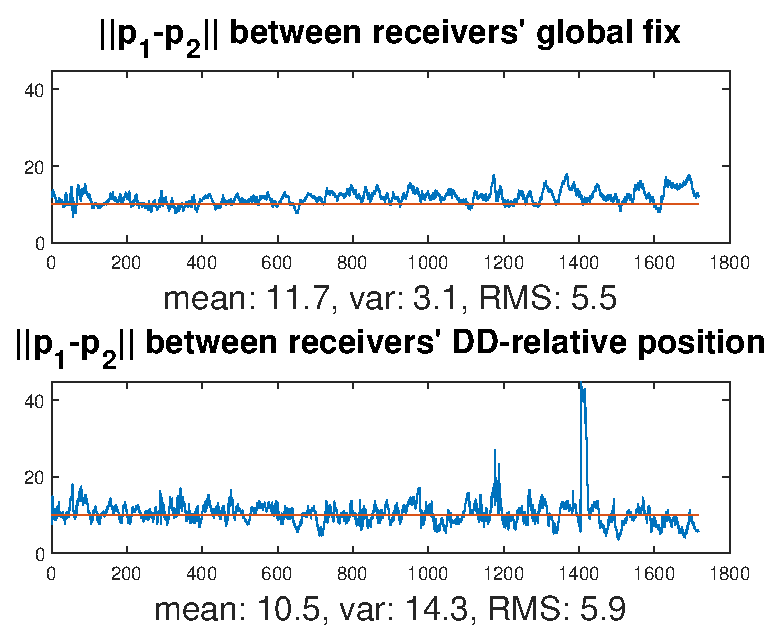
\includegraphics[width=\textwidth]{Results/MSEplots/Eobs.eps}
\subcaption{\label{fig:Eobs} Receivers separated 10 m in east direction.}
\end{subfigure}
\caption{Calculated RMSE of relative position from global position estimator and DD estimator from observation data. Receiver separation as indicated in the respective subcaption.}
\end{figure}

\section{DOP values}\label{sectionDOP}
The DOP-values of the observation series are calculated as presented in section \ref{satelliteGeometry}. The results from the global position and DD-estimator are presented in section \ref{ch:globalDOP} and \ref{ch:DD_DOP} respectively. The DOP values are presented in order to find if any poor performance can be explained by the satellite geometry.

\begin{comment}
In order to evaluate the variance of the estimates, the results of the observations are tied to their respective DOP-values, calculated as described in equations \ref{eq:HDOP} and \ref{eq:VDOP}. An estimate of the UERE values can be calculated from equation \ref{UERE} as 
\begin{align}\label{epsilon}
\epsilon=\frac{\sigma}{q}
\end{align}
The value of $\epsilon$ will be presented as $\epsilon_H$ and $\epsilon_V$, where $\epsilon_H$ is the root sum squared of the $\sigma_N$ and $\sigma_E$ values.
\end{comment}
\subsection{Global position estimator DOP values} \label{ch:globalDOP}
The DOP values from the observation series calculated for the global position estimator are presented in figure \ref{fig:DOP1}-\ref{fig:DOP2}. The values are similar for receiver 1 and receiver 2 which is expected since only the difference in observed satellites should produce a difference in DOP-values with a short baseline distance. The HDOP and VDOP value with a mean of around 0.5 and 2 respectively at N-separation observation, and mean of around 0.45 and 1.6 for the E-separation observation. These are all well within the acceptable range of what can be considered good geometry, as presented in section \ref{satelliteGeometry} and it is unlikely that the high error in the relative estimates from the global position estimator presented in section \ref{RMSEsection} are due to the satellite geometry.
\begin{comment}
Using the information from table \ref{table:resultsPosAllSat}, 
and the relation in equation \ref{epsilon} gives an estimate of the noise level. 
The $\epsilon_H$ and $\epsilon_H$ values are calculated per receiver
\\For the N-direction sample series:
\begin{align*}
\epsilon_{H,1}&=2.4 & \epsilon_{H,2}=5.8\\
\epsilon_{V,1}&=1.2 & \epsilon_{V,2}=1.8
\end{align*}
For the E-direction sample series: 
\begin{align*}
\epsilon_{H,1}&=4.1 & \epsilon_{H,2}=3.9\\
\epsilon_{V,1}&=1.4 & \epsilon_{V,2}=2.0
\end{align*}
\end{comment}
\begin{comment}
ALSSAT
N-DIR
sigma1 1N 0.7E ==> 1.2, 2.4D, eps=1.2/0.5H, 2.4/2=1.2V
sigma2 2N 2.1E==>2.9, 3.5D, eps=2.9/0.5=5.8, 3.5/2=1.8V
E-DIR
sigma1 1.6N, 0.9E ==> 1.8,  2.2D ger att eps=1.8/0.45=4.1H, 1.38V
sigma2 1.2 1.3 ==1.7 3.3D eps= 1.7/0.45=3.9, 3.3/1.6=2.01V

SHAREDSAT
DOP VALUES E:
H: 1.1, V: 4.24
DOP VALUES N:
H: 1.1, V: 3.2
E
sigma1: 1.8N, 1.4E ==> 2.28, 2.5D ger eps=2.28/1.1=2.01, 2.5/4.24=0.5
sigma2: 1.4N, 1.3E ==> 1.91, 3.8D ger eps=1.91/1.1=1.73, 3.8/4.24=0.89
N
sigma1: 1N, 0.7E ==>  1.22, 2.5D ger 1.22/1.1=1.11, 2.5/3.2=0.78
sigma2: 2N, 0.7E ==> 2.12, 3.5D ger 2.12/1.1=1.92, 3.5/3.2=1.09


\end{comment}
\begin{figure}[!h]
\centering
\begin{subfigure}{0.8\textwidth}
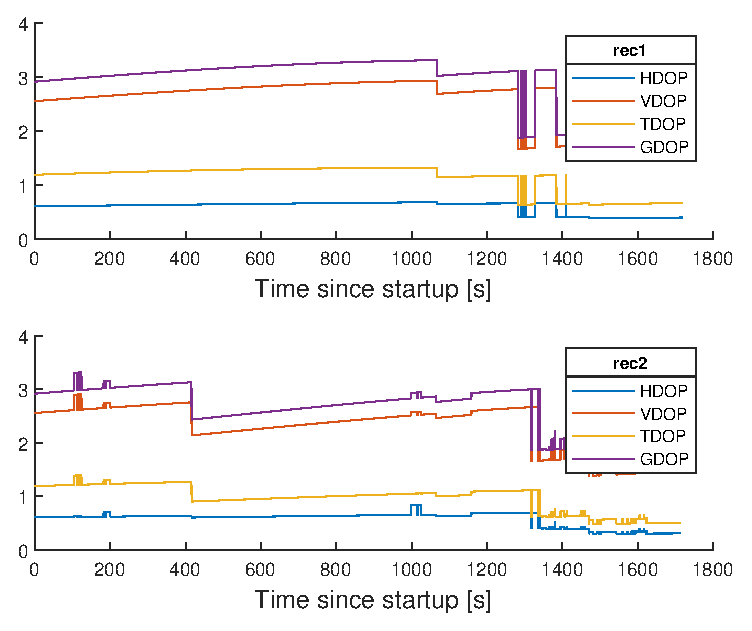
\includegraphics[width=\textwidth]{Results/DOP_N}
\subcaption{\label{fig:DOP1} Receivers separated 10 m in N-direction. Upper: receiver 1. Lower: receiver 2.}
\end{subfigure}
\begin{subfigure}{\textwidth}
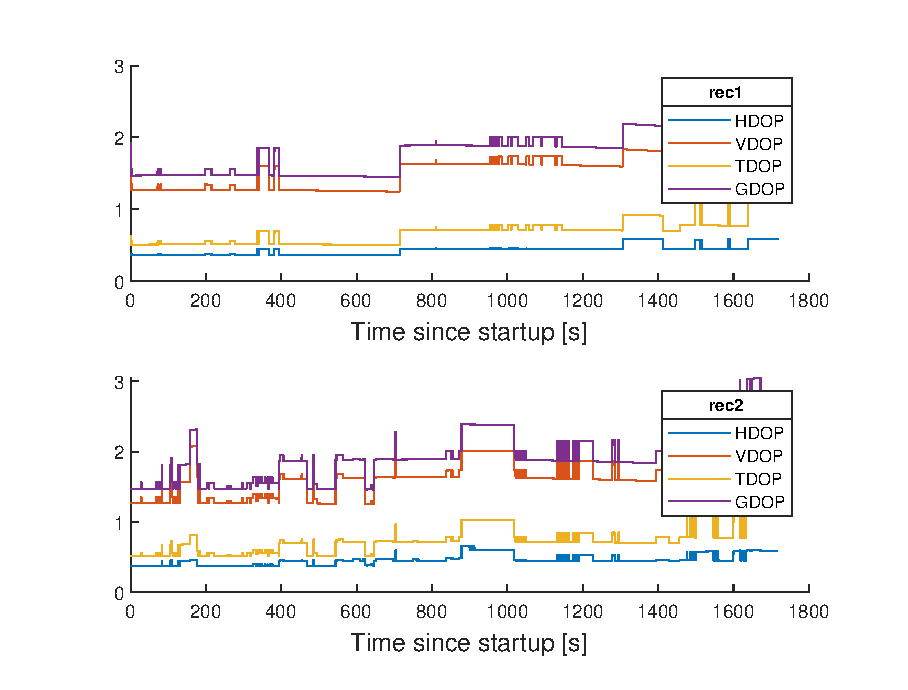
\includegraphics[width=\textwidth]{Results/DOP_E}
\subcaption{\label{fig:DOP2} Receivers separated 10 m in E-direction. Upper: receiver 1. Lower: receiver 2.}
\end{subfigure}
\caption{Individual DOP values for two receivers. Jumps in DOP-value between two epochs are due to change in which satellites are tracked by the receiver.}
\end{figure}

\subsection{Double difference estimator DOP values}\label{ch:DD_DOP}
The DOP-values calculated for the DD-estimator differs from that of section \ref{satelliteGeometry} in that the TDOP-value is not included in the equations. This is due to that the receiver clock bias $\Delta t_{rec}$ is not estimated. This results in the DOP-matrix being reduced to a $3\times3$ matrix. The GDOP value is thus calculated as $$q_G=\sqrt{q^2_H+q^2_V}$$ when the TDOP value is omitted. Besides that, calculations are performed equally.
The calculated DOP-values are shown figures \ref{fig:DD_DOP1}-\ref{fig:DD_DOP2}. The HDOP and VDOP values have a mean of 0.56 for the HDOP and 0.77 for VDOP in the N-direction separated observation, and 0.46 and 0.57 for the E-separated observation. This indicate that the satellite geometry was very good, with the exception of a few samples where it exceeds 3. Similarly to what was mentioned in section \ref{ch:globalDOP}, the satellite geometry is unlikely to be a large factor in explaining the errors in section \ref{RMSEsection}.
\begin{figure}[!h]
\begin{subfigure}{\textwidth}
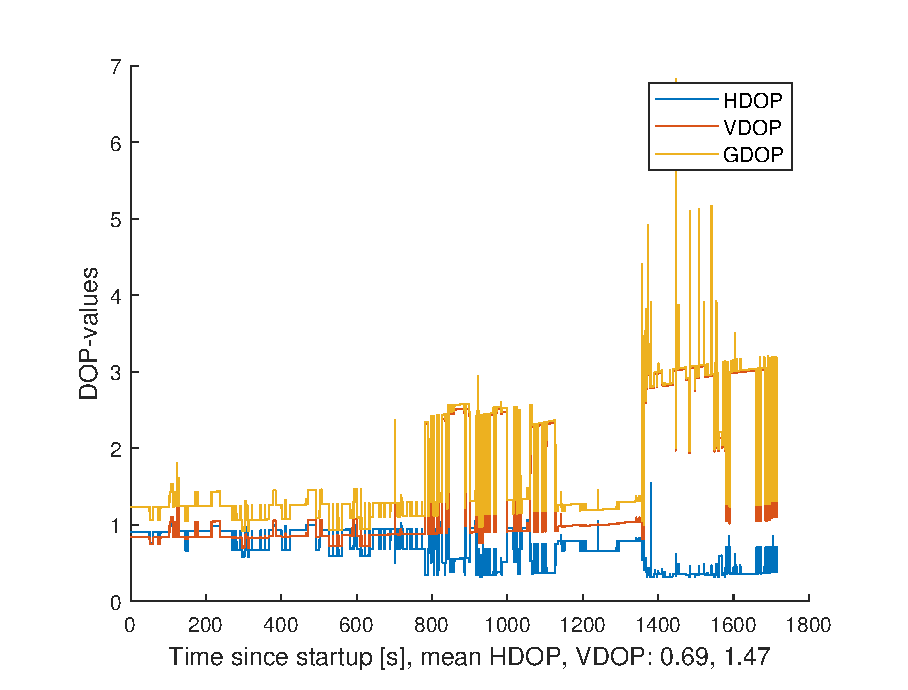
\includegraphics[width=\textwidth]{Results/DDDOPN}
\subcaption{\label{fig:DD_DOP1} Receivers separated 10m in N-direction.}
\end{subfigure}
\begin{subfigure}{\textwidth}
\includegraphics[width=\textwidth]{Results/DDDOPE}
\subcaption{\label{fig:DD_DOP2} Receivers separated 10m in E-direction.}
\end{subfigure}
\caption{DOP values from DD-estimator. Jumps in DOP-values are due to changes in which satellites are tracked by the receivers, as well as a change in which satellite is used as reference.}
\end{figure}

\begin{comment}
Using the values from \ref{table:resultsRel} and equation \ref{epsilon} gives that the calculated values of $\epsilon_H$ is, for the north and east observation respectively equal to 9.26 and 6.35, and $\epsilon_V$ is 10 and 10.2. 

DOP N
H 0.56 V 0.77
DOP E
H 0.46 V 0.57
SIGMA N: 4.3N, 2.9E, 7.7D
SIGMA E: 2.3N, 1.8E, 4.7D
eps_H=9.26 and 6.35
eps_V=10 and 10
\end{comment}
\end{document}
